\documentclass[conference]{IEEEtran}
\IEEEoverridecommandlockouts
\usepackage[T1]{fontenc}
\usepackage{amsmath,amssymb}
\usepackage{graphicx}
\usepackage{booktabs}
\usepackage[numbers,sort&compress]{natbib}
\usepackage{xcolor}
\usepackage[colorlinks=true,linkcolor=blue!50!black,citecolor=blue!50!black,urlcolor=blue!50!black]{hyperref}
\newcommand{\todo}[1]{\textcolor{red}{[TODO: #1]}}
\newcommand{\AffBlurTwo}{0.14}
\newcommand{\AffClutterTwo}{0.23}
\newcommand{\RetBlurTwo}{0.91}
\newcommand{\RetClutterTwo}{0.71}
\newcommand{\AffDarkOne}{0.82}
\newcommand{\RetDarkOne}{0.86}
\newcommand{\AffShiftOne}{0.76}
\newcommand{\RetShiftOne}{0.86}
\newcommand{\TrBlurTwo}{-2.22}
\newcommand{\TrClutterTwo}{-3.51}
\newcommand{\AffMidLo}{0.54}
\newcommand{\AffMidHi}{0.67}
\newcommand{\RetMidLo}{0.77}
\newcommand{\RetMidHi}{0.88}
\newcommand{\HoNewSeen}{1.40}
\newcommand{\HoNewHeld}{4.94}
\newcommand{\HoOrigBoth}{0.76}
\newcommand{\HoOrigHeld}{0.74}
\newcommand{\HoStillHeld}{13.82}
\newcommand{\LbTasks}{10}
\newcommand{\LbEps}{5}
\newcommand{\LbClean}{88}
\newcommand{\LbDark}{74}
\newcommand{\LbBlur}{14}
\newcommand{\LbClutter}{6}
\newcommand{\LbShift}{52}
\newcommand{\PTasks}{6}
\newcommand{\PClean}{83}
\newcommand{\PClutter}{7}
\newcommand{\PImg}{80}
\newcommand{\PImgRec}{0.96}
\newcommand{\POdd}{50}
\newcommand{\POddRec}{0.57}
\newcommand{\PEven}{20}
\newcommand{\PEvenRec}{0.17}
\newcommand{\PText}{3}
\newcommand{\PTextRec}{-0.04}
\newcommand{\OePairs}{30}
\newcommand{\OeOddOnly}{11}
\newcommand{\OeEvenOnly}{2}
\newcommand{\OeP}{0.02}
\newcommand{\OeDiff}{30}
\newcommand{\OeDiffLo}{10}
\newcommand{\OeDiffHi}{50}
\newcommand{\LmFrames}{96}
\newcommand{\LmEpisodes}{10}
\newcommand{\LmLayers}{32}
\newcommand{\LmPooled}{0.47}
\newcommand{\LmWithin}{0.19}


\title{Moved, Not Lost: Locating Appearance-Shift Failures Inside a Small Vision-Language-Action Model}
\author{\IEEEauthorblockN{Tushar Bajaj}
\IEEEauthorblockA{Indian Institute of Technology Bombay\\
\texttt{tusharbajaj2085@gmail.com}}}

\begin{document}
\maketitle
\thispagestyle{plain}\pagestyle{plain}
\raggedbottom

\begin{abstract}
Vision-language-action models (VLAs) degrade when lighting, focus, clutter or camera placement change, but benchmarks report \emph{that} they fail, not \emph{where} inside the model the failure arises. We study SmolVLA, a 450M-parameter VLA, on public SO-101 pick-and-place demonstrations under eight controlled image perturbations. We combine layer-wise representation drift (measured against the natural spread between task moments), linear probes, action comparisons under shared flow-matching noise, and activation patching on the key--value cache through which the action expert reads the backbone. Across 1,510 frames and three seeds we find: (i) drift is set at the vision encoder and passes through all 16 frozen backbone layers essentially unchanged; (ii) gripper state stays linearly decodable (retrained probes reach R$^2$ 0.71--0.91), but under strong blur and clutter even a recalibrated clean probe reaches only \AffBlurTwo{} and \AffClutterTwo{}: the information is re-encoded, not lost; (iii) per-frame drift predicts which \emph{kind} of perturbation is harmful but not which \emph{frame} fails, a Simpson's paradox; (iv) 92--94\% of the action change is carried by image-token keys and values, read through the expert's cross-attention layers, and none by instruction tokens. In closed-loop LIBERO evaluation of the public SmolVLA LIBERO checkpoint, the same perturbations cut task success from \LbClean\% to \LbClutter--\LbDark\%, in the same order as the offline action changes, and restoring the image tokens' keys and values at every control step under clutter raises success from \PClutter\% to \PImg\%. The detailed analyses are offline and cover one model family; closed-loop results use one seed and few episodes. We release code and results.
\end{abstract}

\begin{IEEEkeywords}
vision-language-action models, robustness, interpretability, probing, activation patching
\end{IEEEkeywords}

\section{Introduction}
Vision-language-action models map camera images and a language instruction to robot actions by attaching an action head to a pretrained vision-language model (VLM)~\cite{kim2024openvla,black2024pi0,shukor2025smolvla}. Their brittleness to appearance changes is well documented: systematic benchmarks perturb lighting, textures, camera viewpoints and sensor noise and report large drops in task success~\cite{fei2025liberoplus,guo2025robustvla,xie2026strongvla}. Success rates, however, say only that a policy fails. Practitioners deciding whether to augment training data, replace the vision encoder, fine-tune the backbone or retrain the action head need to know \emph{where} the failure enters the model and \emph{how} it reaches the actions.

\begin{figure*}[t]
  \centering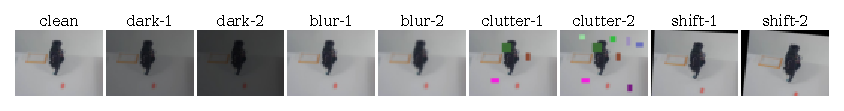
\includegraphics[width=\linewidth]{figures/fig1_perturbations.pdf}
  \caption{One frame (episode 17, frame 40, top camera) under the eight perturbations.}
  \label{fig:pert}
\end{figure*}

We take a mechanistic view of a single, widely used open model, SmolVLA~\cite{shukor2025smolvla}, whose architecture makes the question well posed: a frozen VLM backbone (a SigLIP vision encoder~\cite{zhai2023siglip} and the first 16 layers of SmolVLM2~\cite{marafioti2025smolvlm}) feeds a separately trained action expert that interleaves self-attention with cross-attention to the backbone's key--value (KV) cache, and produces 50-step action chunks by flow matching~\cite{lipman2023flow}. We verify that the deployed checkpoint's backbone is bit-identical to the original VLM, so any appearance sensitivity in the backbone is inherited, and all task-specific learning lives in the action expert.

Our contributions are:
\begin{itemize}
  \item \textbf{A fair drift measure.} Cosine distance reports SmolVLA's representations as 97--99.7\% unchanged under heavy blur because a large component is shared across frames. We instead express the perturbation-induced displacement in units of the typical distance between different clean task moments (``rulers''), separately for the full residual stream and for the backbone layers' own contributions.
  \item \textbf{Localisation.} Drift and representational similarity (CKA~\cite{kornblith2019cka}) are fixed at the vision-encoder output and pass through the 16 frozen backbone layers with at most $-16\%$ to $+11\%$ modulation.
  \item \textbf{Moved, not lost.} Gripper state stays linearly decodable after perturbation. Separating offsets from re-encoding with an affine recalibration of clean-fitted probes, mild dimming and camera shift act mostly as offsets, while strong blur and clutter re-encode the information along new directions that a clean-fitted readout, such as the action expert, cannot use.
  \item \textbf{A negative result guarded against a statistical trap.} Per-frame drift does not predict per-frame action change within any perturbation type; the apparent pooled correlation is a Simpson's paradox~\cite{simpson1951}.
  \item \textbf{Causal routing.} KV-cache activation patching~\cite{meng2022rome,zhang2024patching} shows that the action change is carried by image-token keys and values, read only through the expert's cross-attention layers and distributed across backbone layers 1--11.
  \item \textbf{Closed-loop confirmation.} In LIBERO, the perturbations reduce task success in the same order as the offline action changes, and restoring only the image tokens' KV entries during rollouts restores task success, more through the cross-attention than through the self-attention layers.
\end{itemize}

\section{Related work}
\textbf{VLA robustness.} LIBERO-Plus~\cite{fei2025liberoplus} perturbs object layout, camera viewpoint, robot initial state, language, lighting, background texture and sensor noise in simulation; RobustVLA~\cite{guo2025robustvla} and STRONG-VLA~\cite{xie2026strongvla} study multi-modal perturbations and robust training. Watanabe et al.~\cite{watanabe2026lights} show that illumination augmentation can make a VLA discard colour. These works measure success rates; we measure where in the network appearance changes propagate. Li et al.~\cite{li2025generalizable} attribute viewpoint brittleness to misaligned visual representations and repair it with a learned affine modulation of the visual tokens; our patching and recalibration results give a mechanistic account of why such token-level repairs can work. Our perturbations follow the graded-corruption design of ImageNet-C~\cite{hendrycks2019imagenetc}.

\textbf{Probing VLAs.} Linear probes~\cite{alain2016probes} with control tasks~\cite{hewitt2019control} test what a layer encodes; probe accuracy shows availability, not use~\cite{belinkov2022probing}. Lu et al.~\cite{lu2025probing} probe all OpenVLA layers for object and action states. Closest to us, Act2Answer~\cite{kachaev2026act2answer} probes seven VLAs including SmolVLA, across the backbone and the action expert at every denoising iteration, for answer-relevant knowledge; it does not perturb inputs or measure drift. Jiang et al.~\cite{jiang2026encoded} find that linear probes recover modified instructions from VLA and world-action policies even when those instructions rarely determine which object is picked, a language-side counterpart of the encoded but unusable gripper information we find under appearance change. Embodied Interpretability~\cite{zhang2026embodied} attributes actions to image regions by interventional masking and relates attribution to generalisation. Shen et al.~\cite{shen2026pretraining} compare frozen VLM and video-model features by probing.

\textbf{Causal interventions.} Activation patching and causal tracing~\cite{meng2022rome,zhang2024patching} replace internal activations from one run with those of another to locate the components that mediate a behaviour. Grant et al.~\cite{grant2026features} inject action-expert activations across tasks in six VLAs, including SmolVLA, and find goal binding to absolute workspace coordinates. Wulff and Cangelosi~\cite{wulff2026instructions} apply activation patching to the action modules of $\pi_{0.5}$ and GR00T under corrupted \emph{instructions} and find, for GR00T, sensitivity concentrated in periodic cross-attention layers. Swann et al.~\cite{swann2026causal} patch activations in $\pi_{0.5}$, MolmoAct2 and MolmoBot and find that causally relevant image and instruction information reaches the action expert through a narrow band of mid-to-late cross-attention layers, which they call the action-conditioning interface. Luo et al.~\cite{luo2026lookbefore} report, across several VLAs, that action generation becomes progressively less sensitive to visual tokens in deeper layers. Horiba et al.~\cite{horiba2026detect} use a sparse autoencoder to find a VLA feature that tracks adversarial image patches and suppress it when a linear probe detects an attack. We study natural appearance changes rather than corrupted instructions or adversarial patches: we patch the KV cache that connects a VLA's backbone to its action expert under \emph{appearance} perturbations, offline and in closed loop. Like Swann et al., we find that the effect enters through cross-attention; for appearance perturbations in SmolVLA, however, it is spread over most of the backbone (layers 1--11) rather than concentrated in a narrow band.

\begin{table*}[t]
\centering\small
\caption{Per-perturbation summary. Total drift at layer 0 with 95\% CI; change in update drift from layer 1 to 16; CKA at layer 0 (within 0.004 at layer 16); probe R$^2$ for gripper opening at layer 16 (clean = 0.85): transfer, transfer after affine recalibration, and retrained; action change mean $\pm$ s.d. over three seeds (joint units).}
\label{tab:main}
\begin{tabular}{lccccccc}
\toprule
Perturbation & Total drift & $\Delta$ update & CKA & Transfer R$^2$ & Recal. R$^2$ & Retrained R$^2$ & Action change \\
\midrule
dark-1 & 0.47 [0.47, 0.48] & -16\% & 0.958 & 0.67 & 0.82 & 0.86 & 3.12 $\pm$ 0.02 \\
dark-2 & 0.86 [0.85, 0.87] & +11\% & 0.906 & 0.40 & 0.67 & 0.88 & 4.44 $\pm$ 0.02 \\
blur-1 & 0.85 [0.85, 0.86] & 0\% & 0.860 & -0.34 & 0.65 & 0.88 & 6.10 $\pm$ 0.01 \\
blur-2 & 1.39 [1.38, 1.40] & +6\% & 0.763 & -2.22 & 0.14 & 0.91 & 6.86 $\pm$ 0.01 \\
clutter-1 & 1.01 [1.01, 1.02] & +8\% & 0.822 & -0.10 & 0.54 & 0.77 & 5.48 $\pm$ 0.38 \\
clutter-2 & 1.45 [1.45, 1.46] & +6\% & 0.721 & -3.51 & 0.23 & 0.71 & 7.56 $\pm$ 0.17 \\
shift-1 & 0.69 [0.69, 0.70] & -7\% & 0.890 & 0.73 & 0.76 & 0.86 & 4.49 $\pm$ 0.01 \\
shift-2 & 0.81 [0.81, 0.82] & 0\% & 0.876 & 0.58 & 0.62 & 0.83 & 5.66 $\pm$ 0.01 \\
\bottomrule

\end{tabular}
\end{table*}

\begin{figure*}[t]
  \centering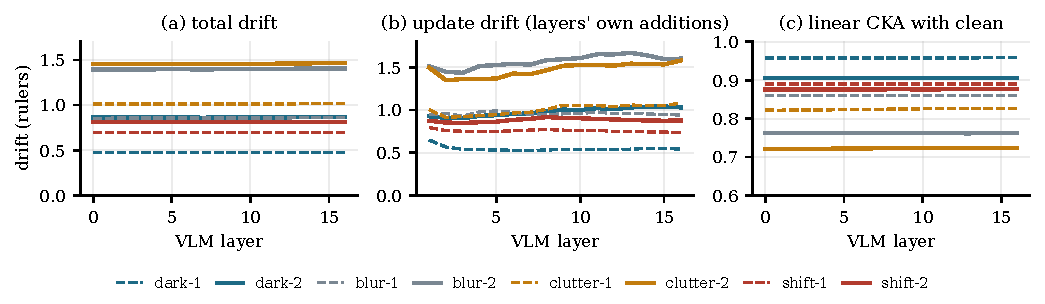
\includegraphics[width=\linewidth]{figures/fig2_drift.pdf}
  \caption{Per-layer (a) total drift, (b) update drift (backbone layers' own contributions; starts at layer 1) and (c) linear CKA with clean features. 1,510 frames, seed 0. Dashed: severity 1; solid: severity 2.}
  \label{fig:drift}
\end{figure*}

\section{Setup}
\subsection{Model and data}
We use the public checkpoint \nolinkurl{dajiangw/smolvla_svla_so101_pickplace_finetune}, fine-tuned from \nolinkurl{lerobot/smolvla_base} on \nolinkurl{lerobot/svla_so101_pickplace} (50 teleoperated episodes, two cameras, 30\,Hz, task ``pink lego brick into the transparent box'') with LeRobot~\cite{cadene2024lerobot}. SmolVLA embeds each 512$\times$512 image into 64 tokens (SigLIP + pixel shuffle + linear connector), appends the instruction tokens and one token projected from the six joint readings, and runs this prefix through the first 16 layers of SmolVLM2 (width 960). The action expert (16 layers, width 720) alternates self-attention (even layers) and cross-attention to the backbone's per-layer KV cache (odd layers; \texttt{self\_attn\_every\_n\_layers}\,=\,2) and integrates a flow-matching velocity field in 10 Euler steps to a 50$\times$6 action chunk (1.67\,s).

\textbf{Which parts were trained?} Comparing weights tensor by tensor, the vision encoder, connector and all 16 backbone layers are bit-identical across the original SmolVLM2, \texttt{smolvla\_base} and the fine-tuned checkpoint (maximum absolute difference exactly 0), consistent with the SmolVLA paper's frozen-VLM recipe~\cite{shukor2025smolvla}. Fine-tuning changed only the state projection (5\% relative norm change) and the action expert and its projections (14--28\%). The attention mask prevents image and text tokens from attending to the state token, so image-token probes cannot read the joint readings directly.

We sample every 8th frame of all 50 episodes (1,510 frames). Action analyses use 300 frames (six spread over each episode).

\begin{figure*}[t]
  \centering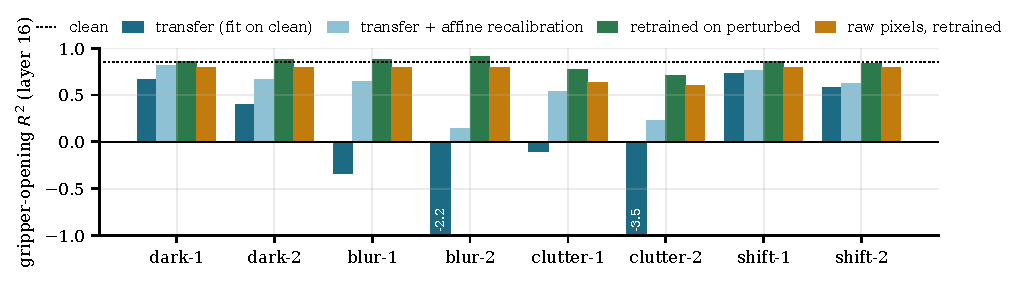
\includegraphics[width=\linewidth]{figures/fig3_probes.pdf}
  \caption{Gripper-opening probes at layer 16 (every layer looks alike). Transfer: fitted on clean frames; affine recalibration: transfer predictions after the best linear rescaling and shift (squared correlation); retrained: fitted on perturbed frames; held-out episodes throughout. Values below $-1$ are clipped and labelled.}
  \label{fig:probes}
\end{figure*}

\begin{figure*}[t]
  \centering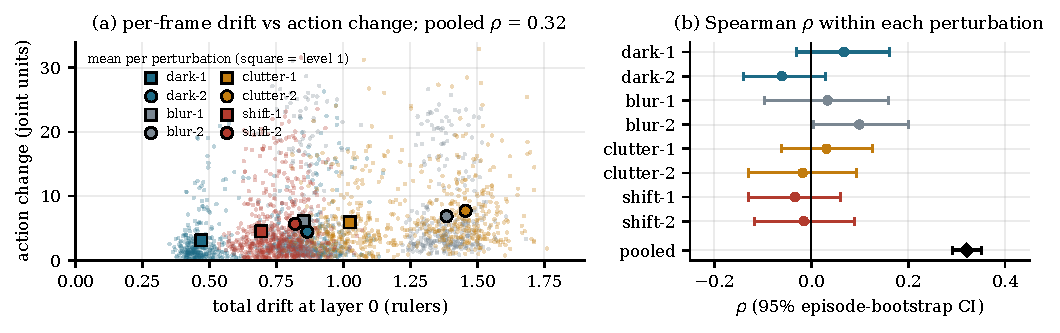
\includegraphics[width=\linewidth]{figures/fig4_simpson.pdf}
  \caption{(a) Per-frame total drift at layer 0 against action change for 300 frames $\times$ 8 perturbations (seed 0); large markers are per-perturbation means. (b) Spearman $\rho$ within each perturbation (95\% episode-bootstrap CI) and pooled.}
  \label{fig:simpson}
\end{figure*}

\subsection{Perturbations}
Eight perturbations (Fig.~\ref{fig:pert}) are applied identically to both cameras at two severities: \emph{dark} (pixel values $\times 0.6$ / $\times 0.35$), \emph{blur} (Gaussian, $\sigma = 2$ / 5\,px at 480$\times$640), \emph{clutter} (3 / 8 solid rectangles of 30--70\,px at seeded random positions) and \emph{camera shift} (translation 5\% / 10\%, rotation 3$^\circ$ / 6$^\circ$, zoom 1.05 / 1.10, black borders). The robot state and instruction are unchanged, so the correct action is unchanged. Rectangles can occlude the gripper, and the affine shift has no parallax.


\subsection{Measurements}
\textbf{Representations.} Forward hooks record the residual stream entering each backbone layer and leaving the last (17 points, point 0 = embeddings after the vision encoder and connector), mean-pooled over each camera's 64 image tokens and concatenated (1,920 dimensions).

\textbf{Drift in rulers.} Mean-pooled image tokens have norm $\approx$3,555 while the backbone layers change them by only 1--14\% (cosine to layer~0 $\geq 0.993$), so cosine distance between clean and perturbed states is only 0.003--0.03. We therefore define, at layer $L$,
\begin{equation}
  d_L(x) = \frac{\lVert h_L(\tilde{x}) - h_L(x) \rVert_2}{\operatorname{median}_{(i,j)} \lVert h_L(x_i) - h_L(x_j) \rVert_2},
\end{equation}
where $\tilde{x}$ is the perturbed version of frame $x$ and the denominator (the ``ruler'') is the median distance over 20,000 random pairs of clean frames from \emph{different} episodes. \emph{Total drift} uses $h_L$; \emph{update drift} uses $u_L = h_L - h_0$, the backbone layers' own contribution, with its own ruler. The total ruler is 910--918 at all layers; the update ruler grows from 5.3 (layer 1) to 83.6 (layer 16). We also report linear CKA~\cite{kornblith2019cka} between clean and perturbed representations over all frames.

\textbf{Probes.} Ridge-regression probes predict gripper opening from image-token representations, with episode-grouped 5-fold cross-validation and the regularisation strength chosen on held-out training episodes. \emph{Transfer} probes are fitted on clean frames and tested on perturbed frames of held-out episodes; \emph{retrained} probes are fitted and tested on perturbed frames. Controls are shuffled labels (R$^2 \approx 0$), a raw-pixel probe (24$\times$32 per camera) and the state token, which trivially decodes gripper opening (R$^2 \approx 1$) because it is a linear function of the joint readings. On clean frames, image tokens reach R$^2 = 0.85$ at every layer, versus 0.79 for raw pixels; a random-frame split inflates this by 0.02.

\textbf{Action change.} For each frame we run the full model on clean and perturbed inputs with the \emph{same} initial flow-matching noise (seeded per frame), so the chunks differ only through the image. Action change is the mean absolute difference over the 50 steps and 6 joints, in the dataset's joint units. We compare clean with perturbed predictions rather than with recorded actions, because the evaluated episodes are part of the fine-tuning set and demonstrations are themselves variable.

\textbf{Activation patching.} The expert reads the backbone only through its per-layer KV cache. For each perturbed frame we build the clean and perturbed prefix caches and denoise from the shared noise with mixed caches: clean values for one token group (both cameras, one camera, or instruction) at all layers, for a single layer, or for layers $0..L$. \emph{Recovery} is $1 - \overline{\lvert a_{\text{patch}} - a_{\text{clean}} \rvert} / \overline{\lvert a_{\text{pert}} - a_{\text{clean}} \rvert}$. Patching nothing and patching everything reproduce the perturbed and clean chunks exactly (difference 0.0).

\textbf{Action expert.} We record the expert's residual stream (17 points, mean over the 50 action tokens) at denoising steps 0, 3, 6 and 9.

\textbf{Statistics and compute.} Confidence intervals are 95\% percentile intervals from 1,000 bootstrap resamples of whole episodes~\cite{efron1993bootstrap}, since frames within an episode share object placement and operator motion. Correlations are Spearman's $\rho$. Seeds 0--2 vary distractor placement and initial noise. All model passes ran in float32 (TF32 disabled) on one NVIDIA L4 GPU; drift values agree with a separate Apple-silicon run within $\approx$1\%, but decoded video differs slightly across platforms ($\approx$0.3\% per pixel), so all compared quantities come from the same platform. bfloat16 inference was rejected because it perturbs activations by $\approx$20\%.

\begin{figure*}[t]
  \centering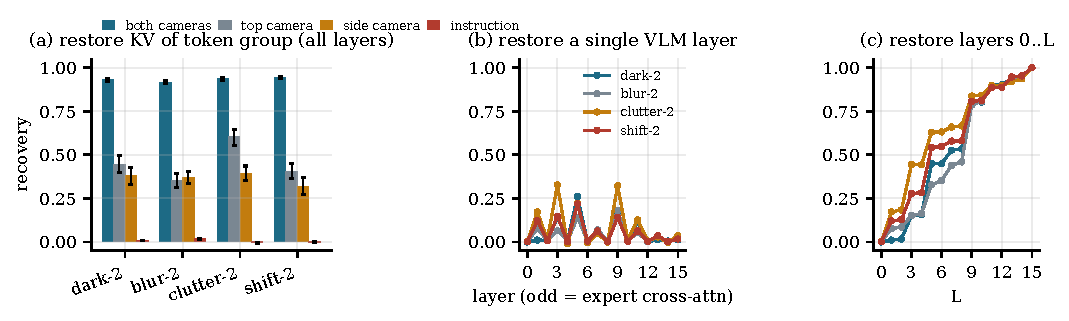
\includegraphics[width=\linewidth]{figures/fig5_patching.pdf}
  \caption{KV-cache activation patching for the four severity-2 perturbations (300 frames, seed 0). Recovery = fraction of the action change removed. (a) Clean KV for a token group at all layers (95\% CI). (b) Clean KV at a single backbone layer. (c) Clean KV at layers $0..L$.}
  \label{fig:patch}
\end{figure*}

\section{Results}

\subsection{Drift originates in the vision encoder and passes through the backbone}
Perturbations displace the image representation by 0.47 (dark-1) to 1.45 (clutter-2) rulers at layer 0 (Table~\ref{tab:main}): under strong blur or clutter a frame moves farther from its clean self than two different moments of the task are from each other. Total drift and CKA are flat across all 17 points (Fig.~\ref{fig:drift}a,c). Update drift, the backbone layers' own contribution, changes between layer 1 and 16 by $-16\%$ to $+11\%$ (Fig.~\ref{fig:drift}b) with intervals of about $\pm 0.01$: small, statistically detectable modulations in both directions, and never a correction. Since the backbone is frozen general-purpose VLM weights, this is not surprising, but it fixes the locus of the problem: whatever the action expert receives is already determined at the vision-encoder output.


\subsection{Task information is moved, not lost}
Clean-fitted probes degrade sharply under blur and clutter (Fig.~\ref{fig:probes}; R$^2$ of \TrBlurTwo{} for blur-2 and \TrClutterTwo{} for clutter-2, i.e.\ worse than predicting the mean), yet probes retrained on the perturbed representations recover 0.71--0.91, so the gripper state remains linearly decodable. A negative transfer R$^2$ could, however, come from a mere offset of the representation along the probe direction. We therefore also report the transfer probe after the best affine recalibration of its outputs, equal to the squared correlation between its predictions and the target. Three regimes appear. For dark-1 and shift-1, recalibration recovers nearly everything (\AffDarkOne{} vs.\ \RetDarkOne{} retrained; \AffShiftOne{} vs.\ \RetShiftOne{}): the perturbation mostly shifts the representation. For dark-2, blur-1, clutter-1 and shift-2 it recovers part (\AffMidLo{}--\AffMidHi{} vs.\ \RetMidLo{}--\RetMidHi{}). For blur-2 and clutter-2 it recovers almost nothing (\AffBlurTwo{} and \AffClutterTwo{} vs.\ \RetBlurTwo{} and \RetClutterTwo{}): the information has moved to directions the clean readout does not use. The raw-pixel control (retrained 0.60--0.80) confirms the image still contains the information, partially occluded under clutter. Because the action expert was trained only on clean images, it is itself a clean-fitted readout of these representations. This parallels image classification, where networks that rely on spurious features still encode the core features, and retraining only the last layer recovers robustness~\cite{kirichenko2023lastlayer}.


\begin{figure}[!t]
  \centering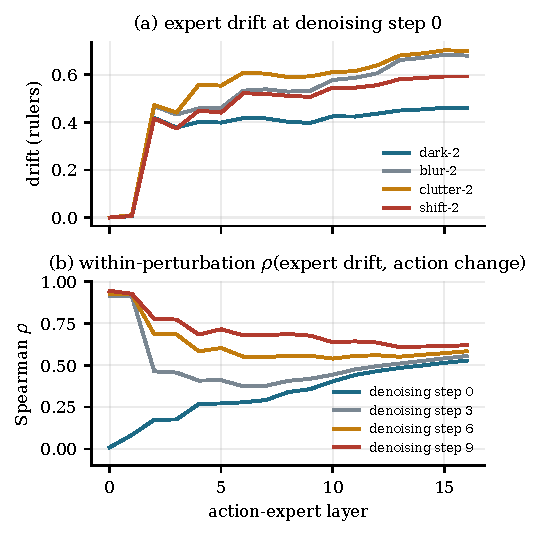
\includegraphics[width=\columnwidth]{figures/fig6_expert.pdf}
  \caption{Action expert. (a) Drift of the expert residual stream at denoising step 0 for the four severity-2 perturbations. (b) Within-perturbation Spearman $\rho$ between expert drift and action change, averaged over the eight perturbations, per denoising step.}
  \label{fig:expert}
\end{figure}

\subsection{Action chunks change, consistently across seeds}
Predicted chunks shift by 3.12 (dark-1) to 7.56 (clutter-2) joint units on average (Table~\ref{tab:main}). For reference, a clean chunk moves the base joint by about 39 units over its 1.67\,s; under clutter-2 the base-joint prediction shifts by about 12. Seed-to-seed standard deviations are at most 0.02 except for clutter (0.17--0.38), whose seed also moves the rectangles.

\subsection{Drift predicts the harmful perturbation type, not the failing frame}
Pooled over the eight perturbations, per-frame drift correlates with per-frame action change ($\rho = 0.32$ [0.29, 0.35]; 0.31 and 0.32 for seeds 1 and 2). Within every perturbation type, however, the correlation is indistinguishable from zero (Fig.~\ref{fig:simpson}b; mean within-type $\rho$ of 0.01, 0.00 and 0.04 for the three seeds). The pooled association arises because blur and clutter produce both more drift and larger action changes than dimming: a Simpson's paradox~\cite{simpson1951}. At the level of perturbation types ($n=8$), mean drift ($\rho = 0.81$) and especially clean-probe failure ($\rho = -0.88$) track mean action change, suggesting that the direction of the displacement, whether it breaks clean readouts, matters at least as much as its size. Raw pixel change does not predict action change ($\rho = -0.16$ [$-0.18$, $-0.13$]).


\subsection{Per-frame failures emerge inside the action expert}
At the first denoising step the expert's input is identical for clean and perturbed frames. Its residual stream stays unchanged through the first (self-attention) layer, drift 0.01, and jumps to 0.42--0.47 rulers after its first cross-attention layer (Fig.~\ref{fig:expert}a), growing to 0.46--0.70 by the last layer. The within-type correlation between expert drift and action change rises with depth from 0.01 to 0.53 (Fig.~\ref{fig:expert}b). At later denoising steps the expert's input is the partially denoised chunk, which already carries the perturbation, so early-layer correlations are high by construction. Whereas backbone drift is uninformative about individual frames, which frames end up with altered actions is determined progressively inside the expert.


\subsection{Patching: image-token keys and values, read through cross-attention}
Restoring the clean KV entries of the image tokens at all layers recovers 0.93, 0.92, 0.94 and 0.94 of the action change for dark-2, blur-2, clutter-2 and shift-2 (Fig.~\ref{fig:patch}a; intervals $\approx \pm 0.01$). Restoring the instruction tokens recovers 0.00 $\pm$ 0.02, although probing shows that text tokens absorb image information within two layers; the expert does not rely on that copy. Each camera alone recovers 0.32--0.60, roughly additively. Restoring a single layer recovers $\le 0.01$ in absolute value at every even layer and 0.01--0.33 at odd layers (Fig.~\ref{fig:patch}b), matching the expert's alternation: perturbation information reaches the actions through cross-attention, not through the self-attention layers that also see the prefix cache. Cumulative restoration rises in steps at odd layers and reaches about 0.9 by layer 11 (Fig.~\ref{fig:patch}c): the effect is distributed rather than concentrated in a single layer, and the last four layers add only about 0.1, consistent with the weaker visual-token sensitivity of deeper layers reported by Luo et al.~\cite{luo2026lookbefore}.


\subsection{Held-out episodes}\label{sec:heldout}
The public checkpoint was fine-tuned on all 50 episodes, so every analysis above uses frames the action expert was trained on. To test whether the findings depend on this, we fine-tuned SmolVLA ourselves from \nolinkurl{lerobot/smolvla_base} on 40 episodes, holding out 10 chosen at random (episodes 2, 16, 19, 24, 25, 26, 30, 31, 32, 48). We kept the public recipe (batch 64, AdamW, learning rate $10^{-4}$ with cosine decay, seed 1000, frozen VLM, no image augmentation, the same camera mapping) except for 15k instead of 100k steps (the public schedule reaches its learning-rate floor at 30k) and mixed-precision training; mixed and full precision gave identical losses in a 300-step check, and the backbone remains bit-identical to \nolinkurl{smolvla_base}. We then repeated the action, expert and patching analyses on 300 frames from the held-out episodes and 300 frames from the training episodes, with the same model.

On identical frames, the public model's open-loop error against the recorded actions is the same on all episodes (\HoOrigBoth{} and \HoOrigHeld{}), because it trained on all of them. Our model's error is \HoNewSeen{} on episodes it trained on and \HoNewHeld{} on held-out episodes, versus \HoStillHeld{} for predicting that the arm stays still (Table~\ref{tab:heldout}). Absolute accuracy therefore depends strongly on memorisation, which is why the check matters. All mechanistic findings, however, replicate on held-out episodes (Table~\ref{tab:heldout}): perturbations change the action chunks with the same ordering; the pooled drift--action correlation again vanishes within every perturbation type; expert drift again predicts per-frame action change by the last expert layer; and patching again attributes the change to image-token keys and values, with no contribution from instruction tokens and recovery only at the expert's cross-attention (odd) layers.

\begin{table*}[t]
\centering\small
\caption{Held-out check. Original study: public checkpoint (trained on all 50 episodes). New model: our 40-episode fine-tune, evaluated on frames from its 40 training episodes (seen) and from the 10 held-out episodes (unseen). $^\dagger$Public model on the same seen / held-out frames; it trained on both.}
\label{tab:heldout}
\setlength{\tabcolsep}{3pt}
\begin{tabular}{lccc}
\toprule
 & Original study & New, seen & New, unseen \\
\midrule
Action MAE vs.\ recorded (same frames) & 0.76 / 0.74$^\dagger$ & 1.40 & 4.94 \\
``Stay still'' baseline MAE & -- & 14.17 & 13.82 \\
Action change, range over 8 perturbations & 3.12--7.56 & 2.37--6.65 & 2.01--6.69 \\
Pooled / mean within-type $\rho$ & 0.32 / 0.01 & 0.28 / -0.02 & 0.35 / 0.04 \\
Expert-drift $\rho$ at expert layer 16 (step 0) & 0.53 & 0.48 & 0.44 \\
Patching recovery: image tokens & 0.92--0.94 & 0.89--0.92 & 0.88--0.92 \\
Patching recovery: instruction tokens & -0.01--0.02 & -0.01--0.00 & -0.01--0.01 \\
Single-layer recovery: odd / even (mean) & 0.08--0.16 / 0.00--0.00 & 0.07--0.12 / 0.00--0.01 & 0.09--0.13 / 0.00--0.01 \\
\bottomrule

\end{tabular}
\end{table*}


\subsection{Closed loop in simulation}\label{sec:libero}
The analyses above measure changes in predicted actions. To test whether these changes cause task failure, and whether the causal path found offline also governs behaviour, we turn to closed-loop evaluation in LIBERO~\cite{liu2023libero}. We use the public SmolVLA LIBERO checkpoint (\nolinkurl{HuggingFaceVLA/smolvla_libero}), which has the same architecture but keeps all \LmLayers{} SmolVLM2 layers in its frozen backbone (the SO-101 checkpoint keeps 16) and reads two cameras. We run LeRobot's official evaluation on LIBERO-Object (\LbTasks{} tasks, \LbEps{} episodes each, fixed initial states) and apply the four severity-2 perturbations to both camera images at every control step; the clutter layout is fixed within an episode.

\textbf{Perturbations cause failure, in the offline order.} Success falls from \LbClean\% (clean) to \LbDark\% (dark-2), \LbShift\% (shift-2), \LbBlur\% (blur-2) and \LbClutter\% (clutter-2) (Table~\ref{tab:libero}). The ranking matches that of the offline action change, both of the SO-101 model (Table~\ref{tab:libero}) and of this checkpoint (Table~\ref{tab:liberomech}): dark $<$ shift $<$ blur $<$ clutter, although the success intervals of blur-2 and clutter-2 overlap.

\textbf{Closed-loop patching.} At every control step we compute the prefix KV cache from both the perturbed and the clean rendering of the same simulator state and let the policy act on the perturbed cache with the clean entries of selected tokens and layers, with one shared noise sample. Without patching, this code path reproduces the official policy's actions exactly (maximum difference 0). The patching runs were stopped early by our compute budget; we compare all recipes on the \PTasks{} tasks completed by every run, on which the unpatched policy succeeds in \PClean\% of clean and \PClutter\% of clutter-2 episodes. Under clutter-2, restoring the image tokens' entries at all layers raises success from \PClutter\% to \PImg\% (success recovery \PImgRec{}, where 1 means clean performance). Restoring them only at the odd layers, which the expert reads through cross-attention, gives \POdd\% (\POddRec{}); only at the even, self-attention layers, \PEven\% (\PEvenRec{}); restoring the instruction tokens at all layers, \PText\% (\PTextRec{}). Pairing the \OePairs{} episodes of each recipe by initial state and clutter layout, odd-layer restoration succeeds where even-layer restoration fails in \OeOddOnly{} episodes and the reverse happens in \OeEvenOnly{} (exact McNemar test, $p = \OeP$; difference \OeDiff{} points, 95\% CI [\OeDiffLo, \OeDiffHi] from a paired bootstrap over tasks). The offline conclusion therefore carries over to task success: the failure travels through the image tokens' keys and values, more through the cross-attention than through the self-attention layers. Unlike on SO-101, restoring the even layers alone is not negligible on this checkpoint (see also Table~\ref{tab:liberomech}).

\textbf{Mechanism on this checkpoint.} During clean rollouts we measured, every 20 control steps, the drift and offline patching recovery for each perturbation (\LmFrames{} frames from \LmEpisodes{} episodes; Table~\ref{tab:liberomech}). Drift is again fixed at the vision encoder and flat across all \LmLayers{} backbone layers; restoring image tokens at the odd (cross-attention) layers recovers most of what restoring them at all layers does, the even layers little; single-layer restorations are small at every layer, as the effect is spread over \LmLayers{} layers, but larger at odd than at even layers; and instruction tokens carry little. Image-token restoration recovers less of the offline action change than on SO-101 (Table~\ref{tab:liberomech}) while recovering almost all of the closed-loop success: small residual deviations need not cause failure. The image and instruction recipes leave the last prefix token, the robot state, perturbed; because it attends to the image tokens, it may carry part of the remainder, which we did not test separately. The pooled drift--change correlation (\LmPooled{}) again exceeds the mean within-type correlation (\LmWithin{}), though here within-type correlations vary in sign across perturbations.

\begin{table}[t]
\centering\small
\caption{Closed-loop success on LIBERO-Object (\LbTasks{} tasks $\times$ \LbEps{} episodes; 95\% CI from a bootstrap over tasks). Top: severity-2 perturbations; drop in points vs.\ clean, and the SO-101 model's offline action change (mean over three seeds, as in Table~\ref{tab:main}) for reference. Bottom: clutter-2 with clean KV entries of the listed tokens and layers restored at every control step, on the \PTasks{} tasks finished by every patching run (on these tasks clean \PClean\%, clutter-2 \PClutter\%); success recovery $=(s-s_\text{clutter})/(s_\text{clean}-s_\text{clutter})$, paired over tasks.}
\label{tab:libero}
\footnotesize
\setlength{\tabcolsep}{1.8pt}
\begin{tabular}{lccc}
\toprule
 & Success (\%) & Drop / recovery & Offline change \\
\midrule
clean & 88 [78, 98] & -- & -- \\
dark-2 & 74 [56, 90] & 14 [-2, 30] & 4.44 \\
blur-2 & 14 [6, 22] & 74 [58, 88] & 6.86 \\
clutter-2 & 6 [2, 12] & 82 [70, 92] & 7.56 \\
shift-2 & 52 [34, 68] & 36 [24, 48] & 5.66 \\
\midrule
\multicolumn{4}{l}{\emph{clutter-2 with clean KV entries for:}} \\
\quad image, all layers & 80 [53, 100] & 0.96 [0.62, 1.40] & -- \\
\quad image, odd (cross-attn.) & 50 [27, 73] & 0.57 [0.30, 0.84] & -- \\
\quad image, even (self-attn.) & 20 [7, 37] & 0.17 [0.00, 0.38] & -- \\
\quad instruction, all layers & 3 [0, 10] & -0.04 [-0.22, 0.09] & -- \\
\bottomrule

\end{tabular}
\end{table}

\begin{table*}[t]
\centering\small
\caption{Mechanism on the LIBERO checkpoint, measured during clean rollouts (\LmFrames{} frames, \LmEpisodes{} episodes). Drift of the mean image-token residual at the encoder output / last backbone layer (rulers); offline action change (normalised action units); offline patching recovery for image tokens at all, odd and even layers and for instruction tokens; mean single-layer recovery at odd / even layers; within-type Spearman $\rho$ between layer-0 drift and action change.}
\label{tab:liberomech}
\begin{tabular}{lcccccccc}
\toprule
Perturbation & Drift L0 / last & Change & Image & Image, odd & Image, even & Text & Single odd / even & $\rho$ \\
\midrule
dark-2 & 0.59 / 0.59 & 0.090 & 0.64 & 0.58 & 0.09 & 0.05 & 0.04 / 0.01 & 0.32 \\
blur-2 & 1.38 / 1.42 & 0.170 & 0.59 & 0.48 & 0.12 & 0.09 & 0.04 / 0.01 & -0.10 \\
clutter-2 & 1.42 / 1.43 & 0.187 & 0.68 & 0.43 & 0.20 & 0.10 & 0.03 / 0.01 & 0.55 \\
shift-2 & 0.94 / 0.94 & 0.162 & 0.74 & 0.65 & 0.08 & 0.06 & 0.04 / 0.01 & -0.00 \\
\bottomrule

\end{tabular}
\end{table*}

\section{Discussion and limitations}
For SmolVLA, the picture is consistent: appearance changes re-encode task information at the vision encoder, the frozen backbone propagates the re-encoding, and an action expert trained only on clean data reads the changed image-token keys and values through its cross-attention layers. Closed-loop patching confirms that restoring the image tokens' cache entries alone restores task success. This suggests, without our having tested a remedy, that remedies belong at the source (a vision encoder or image-token representation stable under appearance change) or in training the action expert on perturbed inputs, rather than in the language layers or any single layer.

The study has clear limits. (1)~The detailed analyses are offline; closed-loop evidence (Sec.~\ref{sec:libero}) comes from a different checkpoint and benchmark, one seed and \LbEps{} episodes per task, and the closed-loop patching comparison from \PTasks{} tasks (\OePairs{} episodes per recipe), so its intervals are wide. (2)~The main analyses use the public checkpoint's training episodes; a held-out replication (Sec.~\ref{sec:heldout}) reproduces every finding, but with only 10 held-out episodes and a model trained for fewer steps. (3)~One model, one task and one scene; models that fine-tune their backbone, such as $\pi_0$~\cite{black2024pi0}, may behave differently. (4)~Perturbations are synthetic: solid rectangles and an affine shift without parallax. (5)~The type-level correlations rest on eight points. (6)~Probes establish availability, not use~\cite{belinkov2022probing}; the causal claims rest on patching alone, and the re-encoding interpretation rests on linear probes and an affine recalibration.

\section{Conclusion}
Tracing eight appearance perturbations through SmolVLA shows that the damage originates in the vision encoder, survives the frozen backbone unchanged, leaves task information intact but re-encoded, and reaches the actions through the image tokens' keys and values at the action expert's cross-attention layers. In closed-loop simulation, the same perturbations cause task failure, and restoring those keys and values restores success. Two methodological points generalise beyond this model: drift must be measured relative to natural between-frame variation rather than by cosine distance, and correlations between internal drift and behaviour must be checked within perturbation types to avoid Simpson's paradox.

\paragraph{Reproducibility} Code, configurations and all result files: \url{https://github.com/TusharBajaj07/smolvla-appearance-shift}. Completed runs used about 8\,GPU-hours on NVIDIA L4 and A10G GPUs (6.3 of them for LIBERO evaluation) and 1.8\,H100-hours for the held-out fine-tune.

\paragraph{Use of AI assistance} Experiment code, analyses, figures and an initial draft of this manuscript were produced with the help of an AI coding assistant (Claude, Anthropic) under the author's direction. The author reviewed the methods, verified results against the saved outputs and references against their sources, and takes full responsibility for the content.

\bibliographystyle{IEEEtranN}
\bibliography{refs}

\appendix
\section{Perturbation and probe details}
Probes use ridge regression on standardised features with $\lambda \in \{10^{-1},\dots,10^5\}$ selected on 20\% of the training episodes; binary gripper-open probes (threshold 10 joint units; clean balanced accuracy 0.95) give the same picture: transfer accuracy falls to 0.50 (chance) for blur-2 and 0.66 for clutter-2, while retrained probes reach 0.88--0.96 under every perturbation. Shuffled-label controls give R$^2 = 0.00$ and balanced accuracy 0.50. Probing the backbone-update component $u_L = h_L - h_0$ alone also decodes gripper opening (R$^2$ 0.81 at layer 1 to 0.86 at layer 16), so the information is refreshed by the backbone even though the total representation is dominated by the encoder output.

\end{document}
